\documentclass[12pt]{report}
\usepackage[a4paper,top=3cm,bottom=2cm, left=3cm, right=2cm]{geometry}
\usepackage[utf8]{inputenc}
\usepackage{listings}
\usepackage{graphicx}
\usepackage{mathdots}
\usepackage{tikz}
\usepackage{booktabs}
\usepackage{pgffor} 
\usepackage{float}
\usepackage{graphics} 
\usepackage{fancyhdr}
\usepackage[square, sort, numbers]{natbib}
\usepackage{color}
\usepackage{indentfirst}
\usepackage{epigraph}
\usepackage{ragged2e}
\usepackage{blindtext}
\usepackage{amsmath,amsthm,amssymb}
\usepackage{tabto}
\usepackage{pgfplots}
\usepackage{changepage}
\usepackage{subcaption}
\usepackage{fancyvrb}
\usepackage{caption}
\usepackage{minted}
\usepackage{placeins} % put this in your pre-amble
\usepackage{flafter}  % put this in your pre-amble

\usetikzlibrary{patterns}
\usetikzlibrary{arrows.meta}
\usetikzlibrary{positioning,shapes.multipart,shapes}
\graphicspath{{images/}}

\definecolor{mycolor}{RGB}{30,75,180}
\definecolor{mycolor2}{RGB}{40,75,90}
\definecolor{red}{RGB}{200,0,0}
\usepackage[colorlinks = true,
            linkcolor = mycolor,
            urlcolor  = mycolor,
            citecolor = mycolor,
            anchorcolor = mycolor]{hyperref}

\usepackage[hypcap=true,font={small,it}]{caption}
\usetikzlibrary{calc}

\captionsetup{belowskip=2pt,aboveskip=2pt}

\bibliographystyle{abstract}

\renewcommand{\chaptername}{}

\renewcommand{\figureautorefname}{figure} % lower case default ref
\renewcommand{\tableautorefname}{table} % lower case default ref
\let\oldchapter\chapter% Store \section in \oldsection
\renewcommand{\chapter}{\cleardoublepage\oldchapter}% Prepend new \section with \cleardoublepage

\newcommand{\latex}{\LaTeX\xspace}
\newcommand{\mcite}[1]{\textcolor{mycolor}{\citeauthor{#1} (\citeyear{#1})}}
\newcommand{\hcite}[1]{(\textcolor{mycolor}{\citeauthor{#1}, \citeyear{#1}})}
\newcommand{\defi}[1]{\textbf{#1}}
\newcommand{\naming}[1]{\textbf{#1}}
\newcommand{\todo}[1]{\textbf{\color{red} TODO: #1}}
\newcommand{\gam}[2]{\mbox{$\{#1\:|\:#2\}$}}
\newcommand{\Gm}[1]{\mbox{$G#1$}}
\newcommand{\Hm}{\mbox{$H\,$}}
\newcommand{\colorset}{\mbox{$\zeta\;$}}
\newcommand{\ramGraph}[1]{\mbox{$r(#1)$}}

\newenvironment{claim}[2]
	{\begin{adjustwidth}{3em}{3em}
     \noindent\underline{Claim #1}\ignorespaces#2
     \ignorespaces
	}
	{\end{adjustwidth}}

\newenvironment{version}[2]
{\begin{adjustwidth}{2em}{2em}
		\noindent\underline{Version #1}\ignorespaces#2
		\ignorespaces
	}
	{\end{adjustwidth}}

\definecolor{purple2}{RGB}{218,112,214}

\pgfplotsset{style thermograph/.style={
		axis x line*=none, axis y line*=none,
		axis line style={draw=none},
		y label style={rotate=-90,at={(current axis.north west)}, right=5mm},
		ylabel = \textbf{t},
	}
}
\lstset{
	columns=fullflexible,
	mathescape=true,
	numbers=none,
	stepnumber=1,
	morekeywords={return, if, else,  while, vector, using, include, class,
		true, false, function, or, public, private},
	xleftmargin=4.0ex,
	tabsize=4,
	frame = single
}

\lstdefinelanguage{json}{
	basicstyle=\normalfont\ttfamily,
	stepnumber=1,
	numbersep=8pt,
	showstringspaces=false,
	breaklines=true,
	frame=lines,
	backgroundcolor=\color{background}
}

\usepackage{listings}
\usepackage{xcolor}
\colorlet{punct}{red!60!black}
\definecolor{background}{HTML}{FAFAFA}
\definecolor{delim}{RGB}{20,105,176}
\colorlet{numb}{magenta!60!black}

%----------------------------------------------------------------------------------------------------%

%--------------------------------------------- DOCUMENT ---------------------------------------------%
\begin{document}
	\newpage
    \begin{titlepage}
\begin{figure}[H]
    \hspace*{-1.0cm}
    \vspace*{-0.5cm}
    
\includegraphics[scale=1]{images/logo_rit.jpg}\\
\end{figure}

\begin{center}
    \vspace*{2cm}
    
    {\LARGE \textbf{Online Ramsey Theory in Planar Graphs} \\ Independent Study Final Report}
        
	\vspace{1cm}
	 by
    \vspace{1cm}
    
   Matheus Tararam de Laurentys
\end{center}

\vspace{1cm}

\begin{center}   
	{\large Independent Study Report \\ 
		CSCI0599 - Computer Science Undergraduate Independent Study} \\
	\vspace{0.5cm}
	Directed to professor Stanis\l{}aw P. Radziszowski and professor Elouise Oyzon\\
	
\end{center}

\vspace{1cm}

\begin{center}
	Report submitted in partial fulfillment of the\\
	requirements for the independent study course

	\vspace{1.0cm}
	at
	\vspace{1cm}
	
	Rochester Institute of Technology \\
	Department of Computer Science \\
	December 2021
\end{center}

\end{titlepage}
    
    \chapter*{Introduction} 
    The Online Ramsey Game is played alternately between two players, called Builder and Painter, on a graph that is not complete. In their turns, the Builder creates an edge and the Painter paints it. Builder's objective is to create a monochromatic subgraph that is isomorphic to a target graph and Painter's objective is to avoid it as long as possible. The Ramsey Theorem, from which the game is named after, guarantees that if there are enough vertices and the Builder is able to choose edges freely, then he/she always wins, regardless of the target.

Some of the interesting questions come from trying to parameterize the number of moves needed by the Builder and the amount of colors for him/her to win. Other problems arise from limiting rules added to the ones listed above. Consider a class of graphs $\mathcal{G}$, a graph $G$ in $\mathcal{G}$ and a target graph $H$. It is interesting to know whether there exists a sequence of moves starting on $G$ such that all board states $(G_1, \ldots, G_n)$ are inside $\mathcal{G}$ and $H$ is isomorphic to a subgraph of $G_n$. A second question is to define a strategy for the Builder to win for given $\mathcal{G}, G$ and $H$.

This is an independent study proposal. The following text provides some more information about the area of interest, outlines a specific problem, provides the method and schedule for the study and lists intended deliverables. It ends by providing a suggestion of method to evaluate the work done. The sponsor of this Independent Study is Dr. Stanisław P. Radziszowski. The credits of this Independent Study will count towards Advanced Electives.
    
    \chapter*{Online Ramsey Theory}
    Ramsey Theory follows an interesting theorem stating that for any positive integers $r$ and $s$, there is a least positive integer $R(r,s)$ such that every blue-red edge coloring of $K_{R(r,s)}$ has a blue clique with $r$ vertices or a red clique with $s$ vertices. One extensively studied problem is calculating such $R(r,s)$ which proves to be very hard, even for very small values of $r$ and $s$. 

The relation of any blue-red edge coloring of a graph $G$ having either a blue clique of size $r$ or a red clique of size $s$ is denoted by $G\rightarrow(r,s)^e$. Similarly defined, if every edge coloring of $G$ has either a blue copy of $H$ or a red copy of $F$, then $G\rightarrow(H,F)^e$. In a special case, where $H$ is isomorphic to $F$, the \textit{Ramsey Arrowing} is denoted by $G\rightarrow(H)^e$. Another set of problems arise when considering the online version of the problem.

\subsection*{On-line Ramsey Theory\cite{1}}

The word ``online" means that, when checking if $G\rightarrow(H)^e$, the edge coloring of $G$ takes place before the entirety of $G$ is known. The typical way, introduced by \textit{Online Ramsey Theory}\cite{1}, to present the online version of the problem is through a combinatorial game between painter and builder:

\begin{adjustwidth}{2em}{2em}
	\noindent\underline{Online Ramsey Game:}
	Take an unbounded set of vertices with no edges and a target graph $H$. Builder selects two disconnected vertices and adds an edge between them. Following, Painter colors the introduced edge. If a monochromatic copy of $H$ is ever created, then the Builder wins. Painter wins if it provides a strategy to avoid $H$ indefinitely.
\end{adjustwidth}

If the builder provides the edges of $G$, and $G\rightarrow(H)^e$, then the builder wins, because there is no possible way to paint the edges of $G$ while avoiding $H$, as defined above. However, it is not true that if the painter cannot prevent $H$, when given edges of $G$, then $G\rightarrow(H)^e$. The mismatch comes from an additional challenge the painter faces on the online version. The added challenge of the online version comes from the lack of information when the Painter takes its decisions.

Consider now a slightly different version. In this version, the builder can only create graphs belonging to a class of \mbox{graphs $\mathcal{G}$.} Considering that $H \in \mathcal{G}$, $H$ is called unavoidable if the builder can force the painter to create a monochromatic copy of $H$, and called avoidable otherwise. If every graph of a class is unavoidable, then the class is called self-unavoidable.

Together with the formulation of these problems the authors show\cite{1} that the class of forests is self-unavoidable, also mentioned in the second section. For this proof, check the visualization featured in the application or in the original paper. An important comment on this self-unavoidability and the difference between the online and offline version of the problem is that forests are clearly avoidable in the offline version.

On the offline version, in fact, it is possible to avoid $P_4$ by following a simple strategy. Elect roots for all the trees in the forest. Color blue all the edges with odd distance to the root and red those with even distance. This strategy does not work in the online version because the distances to a root are not known at the time they are created by the builder.

When concluding their paper, the authors conjecture that the class of outerplanar graphs is exactly the class of unavoidable graphs when playing with $\mathcal{G}$ as the planar graphs.

\subsection*{Online Ramsey Theory for Planar Graphs\cite{3}}

Ten years later, Šárka Petříčková\cite{3}, proved the conjecture wrong. She showed that the builder can force all outerplanar graphs, but can also force some graphs that are not outerplanar. She proved that all outerplanar graphs are unavoidable, but, then, showed a class of graphs, that is not outerplanar, but that is unavoidable when playing on the planar graphs.

Although the proofs contain too many details to be adapted here, it is worth bringing counter examples of the conjecture. First she shows that even cycles are unavoidable. Then, she shows a strategy, based on structures consisting of even cycles, and adds edges and vertices to the graph in a way that the target graph is reached. The class of non-outerplanar graphs used by her is the class of $\theta_{i,j,k}$ with $i, j$ and $k$ even. A graph denoted by $\theta_{i,j,k}$ is composed of three internally disjoint paths of lengths $i,j$ and $k$. The graphs $\theta_{2,2,2}$ and $\theta_{2,2,4}$:

\begin{center}
	\begin{minipage}{0.55\linewidth}
		\hspace{0.5cm}
	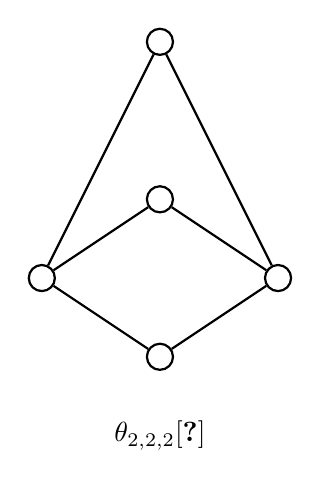
\begin{tikzpicture}[node distance={15mm}, thick, main/.style = {draw, circle}] 
		\node (title) at (1.5, -2) {$\theta_{2,2,2}$\cite{6}};
		\node[main] (1) at(0, 0) {};
		\node[main] (2) at(1.5,1) {}; 
		\node[main] (3) at (1.5, 3) {};
		\node[main] (5) at (3, 0) {}; 
		\node[main] (6) at(1.5,-1) {};
		\draw (1) -- (2);
		\draw (1) -- (3);
		\draw (1) -- (6);
		\draw (2) -- (5);
		\draw (6) -- (5);
		\draw (3) -- (5);
	\end{tikzpicture}
	\end{minipage}
	\begin{minipage}{0.35\linewidth}
	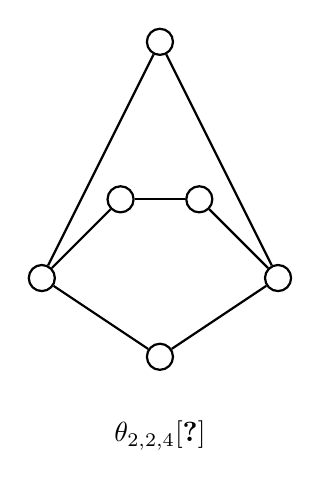
\begin{tikzpicture}[node distance={15mm}, thick, main/.style = {draw, circle}] 
		\node (title) at (1.5, -2) {$\theta_{2,2,4}$\cite{3}};
		\node[main] (1) at(0, 0) {};
		\node[main] (2) at(1,1) {}; 
		\node[main] (3) at (1.5, 3) {};
		\node[main] (4) at (2, 1) {}; 
		\node[main] (5) at (3, 0) {}; 
		\node[main] (6) at(1.5,-1) {};
		\draw (1) -- (2);
		\draw (1) -- (3);
		\draw (2) -- (4);
		\draw (1) -- (6);
		\draw (6) -- (5);
		\draw (3) -- (5);
		\draw (4) -- (5);
	\end{tikzpicture}
\end{minipage}
\end{center}

Are clearly not outerplanar, however it is possible for the builder to force a monochromatic copy of it on the class of planar graphs. Starting from a base structure composed of even-length cycles, showed in gray, the builder just have to build the edges of the graphs below, in black, extracted from Petříčková's work. 

\begin{center}
	\begin{minipage}{0.4\linewidth}
	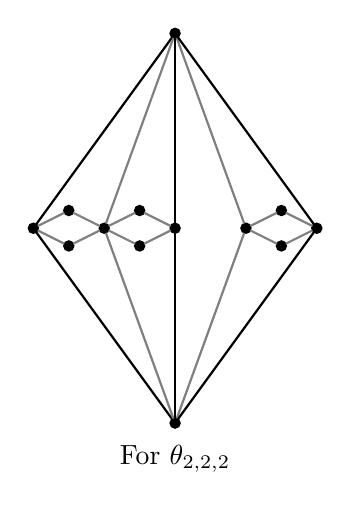
\begin{tikzpicture}[thick, main/.style = {draw, circle, fill=black,scale=0.35}, scale=0.45]
		\node (title) at (4, -6.5) {For $\theta_{2,2,2}$};
		\node[main] (1) at(0, 0) {};
		\node[main] (2) at(1,0.5) {}; 
		\node[main] (3) at (1,-0.5) {};
		\node[main] (4) at (2, 0) {}; 
		\node[main] (6) at(3,0.5) {};	
		\node[main] (7) at(3,-0.5) {};
		\node[main] (8) at(4,0) {};
		\node[main] (9) at(4,-5.5) {};
		\node[main] (10) at(4,5.5) {}; 
		\node[main] (11) at(6,0) {};
		\node[main] (12) at(7,-0.5) {};
		\node[main] (13) at(7,0.5) {};
		\node[main] (14) at(8,0) {};
		\draw[gray] (1) -- (2);
		\draw[gray] (1) -- (3);
		\draw[gray] (2) -- (4);
		\draw[gray] (3) -- (4);
		\draw[gray] (4) -- (6);
		\draw[gray] (4) -- (7);
		\draw[gray] (6) -- (8);
		\draw[gray] (7) -- (8);
		\draw (1) -- (9);
		\draw (1) -- (10);
		\draw (8) -- (9);
		\draw[gray] (9) -- (4);
		\draw[gray] (10) -- (4);
		\draw (8) -- (10);
		\draw[gray] (9) -- (11);
		\draw[gray] (10) -- (11);
		\draw[gray] (11) -- (12);
		\draw[gray] (11) -- (13);
		\draw[gray] (12) -- (14);
		\draw[gray] (13) -- (14);
		\draw (9) -- (14);
		\draw (10) -- (14);
	\end{tikzpicture}
\end{minipage}
	\begin{minipage}{0.4\linewidth}
		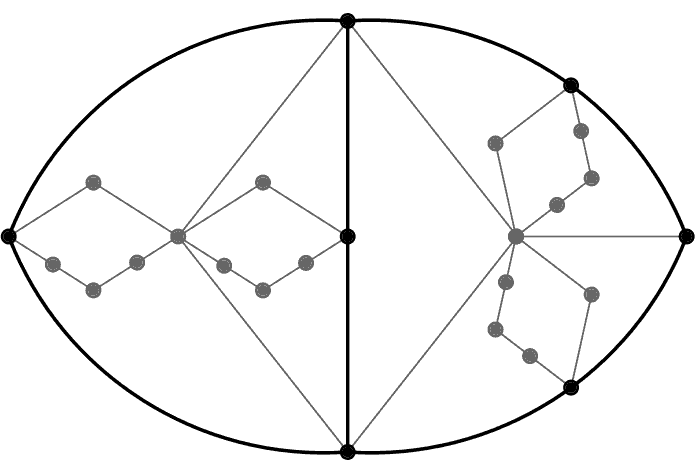
\includegraphics[scale=0.4]{images/theta_2_2_4.png}
		\captionof*{figure}{\hspace{0.7cm}For $\theta_{2,2,4}$}
	\end{minipage}
\end{center}

Petříčková finishes her paper by bringing to light the question whether the class of planar graphs is self-unavoidable, but conjecturing that $K_4$ is avoidable. Of course that if her conjecture is right, then the class of planar graphs is not self-unavoidable. Since 2014, however, no direct progress has been made when it comes to planar graphs, but there are some developments studying other classes.

\subsection*{Online Ramsey theory for a triangle on $F$‐free graphs\cite{3}}

In this paper there is a small shift from what has been highlighted so far. Firstly, it deals with non-planar planar graphs. Secondly, and more importantly, instead of taking a class and deciding whether it is self-unavoidable, the authors take a structure, $C_3$ and study the classes where it is unavoidable. The paper is concerned with classes of graphs where a determined structure is not a subgraph.

First, the authors show that $C_3$ is unavoidable in the class of $K_4$-minor-free graphs. A graph $G$ is a minor of another graph $H$ if, after a sequence of vertex deletions and edge removals or contractions, $G$ is obtained from $H$. This way, $K_4$-minor-free graphs are those for which $K_4$ is never obtained after a sequence of such operations. The result obtained by the authors directly extend the result proved on \textit{On-line Ramsey Theory}.

In the paper from 2004, the authors show that $C_3$ is unavoidable in the class of outerplanar graphs. This means they showed $C_3$ is unavoidable in the class of ($K_{2,3},K_4$)-minor-free graphs. This extension shows that $K_{2,3}$ is not necessary to force a triangle.

Following up, the paper presents a total of five graphs $X_1, X_2. X_3, X_4$ and $X_5$, the larger ones having six vertices. The authors claim and prove that, if a graph $F$ has no isolated vertex and is not isomorphic to $X_5$, then:
\begin{center}
Painter wins the Online Ramsey Game for $C_3$ on the class of $F$-free graphs\\$\iff$\\$F$ is isomorphic to a subgraph of either $X_1,X_2,X_3$ or $X_4$\footnote{This is specially nice because these graphs have between five and six vertices.}
\end{center}

Then, they end their paper by highlighting the only missing result for $C_3$ for such classes of graphs in Online Ramsey Games: ``Who wins the Online Ramsey game for $C_3$ on $X_5$-free graphs"?

\subsection*{One more problem}

When changing the offline problem to the online version, the Painter becomes much weaker. To balance that, restrictions are added to the Builder as well, in the form of restricting its moves to certain classes of graphs. Another option, however, would be making the painter stronger.

For this version, instead of using an unbound set of vertices, the builder has a finite number in its disposal. Additionally, consider that instead of coloring each edge in sequence, the Builder builds $k$ edges in each turn. When the Painter has to make its decisions, it has more knowledge of the overall structure. However, it is not clear whether it is meaningful or not. It actually turns out that this boost is not very meaningful\cite{7}. \textit{Ramsey games against a one-armed bandit} analyzes the problem thoroughly and, although very different from the algebraic approach presented in the other references, complements nicely the study on Online Ramsey Theory. 





    
    \chapter*{Visualization Tool}
    The tool developed during the semester draws simulations using graphs, specified in JSON format, in a canvas. The drawing and canvas interaction part of the application are accomplished using the cytoscapejs library while the interface and simulation functionality were developed specifically for this project. The tool has limited user customization options, but allows the drawing of any graph using a pre-defined layout algorithm.

\subsection*{Simulation specification}

The simulation used by the application is specified via JSON using the following schema:

\begin{lstlisting}[language=json,firstnumber=1,escapechar=*]
{
	"title": "Title displayed on page",
	"description": "Description showed together with title",
	"steps": [
		{
			"graph": "String representation of graph using graph6*\footnote{Compact representation of graphs via strings. Format created by Brendan McKay. Find the specification at https://users.cecs.anu.edu.au/$\sim$bdm/data/formats.txt.}* format.",
			"colors": "color of each edge in the graph, in the order used in the upper triangle of the 'graph'. Specified with a sequence of characters between 'r' (red),  *\mbox{'b' (blue)}*, 'g' (gray) and 'w' (white).",
			"title": "Step title",
			"description": "Step description.",
			"duration": [0-9]+ //seconds the current step is displayed
		},
		*$\cdots$*
	]
}
\end{lstlisting}

The app uses the schema above to create a visualization of the theorem proving that forests are self-unavoidable in the Online Ramsey Game\footnote{More details on the next section.}. The JSON string of this simulation is found on the side menu of the application.

\subsection*{Technologies used}

The app was developed using \texttt{Nodejs}, is implemented in \texttt{TypeScript} and is based on \texttt{React} and \texttt{Redux} frameworks. The conversion to static HTML and JavaScript is done via \texttt{webpack}. The code has the most typical view/component/store architecture. There is no connection to backend services or databases. The app is available on this study's github page\footnote{https://github.com/MLaurentys/IS\_ramsey.}.

\subsection*{Future developments}

One of the important steps forward is improving the graph definition on the simulation JSON file. Using graph6 or another common string formatting is adequate but there is no good online tools for drawing graphs and getting their strings. \textit{House of graphs\footnote{Find more on https://hog.grinvin.org/}} has one built-in but it is limited is some regards. It only shows a limited number of character of the string conversion (being useless for graphs with over ~20 vertices) and the querying of graphs drawing destroys the current canvas, meaning similar queries involve a lot of repeated drawing.

A good way to improve the graph definition is developing the graph6 functionality of the application further. Allowing a similar drawing style to that of House of Graphs but with real-time graph6 conversions would solve most of the issues creating new simulations. However, the problem of specifying the edge colors would remain. To solve that, the app should also display the order of edges or allow for coloring via canvas, with a similar style of real-time conversion.

Another necessity is improving the layout algorithm choices. Neither cytoscapejs nor other graph drawing frameworks have layout algorithms that guarantee drawings of planar graphs without crossing edges. Implementing such algorithms for the main libraries would be a good step forward to make the simulation better. Another related improvement is allowing the user to pick a layout in the simulation specification.









    
    \chapter*{Lessons Learned}
    I wrote the Undergraduate Thesis for my bachelors degree during 2020. It was my first formal research/scientific essay. In the beginning of the year, I decided to give it my best and experience the most, because I would probably not have another chance to try it out, specially with an advisor. I was lucky enough to choose a topic I ended up loving. I spent around five months studying very hard and implementing a lot of ideas I read about. I got a rough sketch of everything I wanted to discuss in my essay in June and started working on the essay soon after.

By November I had a decent looking draft which had all the content I wanted to develop and it was around 80 pages long. I spent the next 2 months revising and improving the text and, although I ended up adding some more content, I got to shrink it to 71 pages. I loved working on it and was very happy that my advisor and the grading committee liked it as well. During the work, that lasted 13 months, I do not remember getting stuck or unfocused.

Leading up to this semester I wanted to do more of that. I reached out to a few professors at RIT and I was very hopeful of working with my current advisor, Stanis\l{}aw P. Radziszowki. Due to academic requirements, the initial research plan was revised to reserve half of the semester to developing a visual tool, which was not exactly what I wanted to do, but I did not mind that.

Focusing on the second half of the semester, I believe that a first mistake I made was in my expectations. I remember thinking that I had a very easy time writing and, unlike my thesis, I would not be starting from scratch: I already knew the proper tools, how to draft a plan that works for me, how to organize references, take good notes an so on. I thought the only missing piece was the knowledge, so after starting learning, I would be ready to start writing.

There were two anticipated text deliveries this semester, but the first one got merged into this final report due to my inability to write it. I cannot pinpoint exactly what the problem was but I will list what I believe major factors were. Unlike with Combinatorial Game Theory, that has didactic materials and books that cover all the developments in the field except for some bleeding edge changes, Ramsey Theory is much more opaque.

In one side I had \textit{Winning Ways}, a gem containing every basic idea there is to know presented in a brilliant manner, and on the other \textit{Combinatorial Game Theory} by Aaron Siegel, which formalized every topic and had the notation used essentially everywhere else. Not only that but there was also CGSuite, by Siegel again, that gave visuals and calculations for every prototype or idea I had. This semester was a different process, where I was reaching out for information scattered across papers, that used different notations and terminologies.

Although I believe I learned a lot and was introduced to interesting and fun subjects, the content did not have time to sink in. When writing, this played the role of making me scared of producing false statements or incorrectly quoting authors. I second guessed some decisions I took and ideas I had. It definitely slowed down the process of writing the essay.

For the same reason it was difficult to produce steady progress. There were times when I understood a new idea, maybe in a proof for a theorem, and that just threw a piece I was developing out. This was progress, in the sense that I learned, but was a slow down in the sense that I did not produce anything. This happened once when I was studying the problem of making the painter stronger by increasing the number of edges before coloring and again when I described the work by Šárka Petříčková.

The problems making progress during the middle of the semester led me to the biggest issue I had. Writing the status report became a burden. I found myself constantly thinking about it, but when I sat down to produce I did not have the words or the ideas necessary to make something of reasonable quality. I want to highlight that my advisor never pressured me. He was always understanding and supportive, at times even reassuring about some ideas I wanted to discard. However, I really wanted to have something to show for.

While having disappointments, I know a bit more now about myself and my relation with writing scientific texts. A first lesson is how valuable a general solid understanding of a field is. Usually, because I write about what I know best, I overlooked the fact that, knowing some theorems and notations does not mean you can write a cohesive and interesting text about a subject. There tends to be more to the ideas connecting theorems than the sum of their results.

A second lesson I take is that I am bad at writing on demand. I am usually great with deadlines and become more productive the more urgent something becomes, but it seems I write the best when I am calm. Following up there an advice my advisor gave me early on but which I did not follow. When developing the app he told me to start writing, but I, instead wanted to finish the app as soon as possible. If I had started earlier I would bump into the knowledge holes earlier and get more time to mature my questions.

It does seems starting to write as early as possible is good because, like in software development, you only notice you have questions when you try to do it yourself. I feel weird now about not following the advice, because it does seem very obvious. A fourth lesson is the value a good book has. I always appreciated books, because I am very focused and get a lot from every one I read. Not having them, though, makes it even more evident. There are other lessons, but I think I brought to light the most meaningful to me right now.

To finalize the text I believe I should say I am happy to have taken this class. Although it came with quite some mental burden, which I described abundantly, I loved the experience and I am forever glad I had this experience sooner rather then later. The end results are not what I hoped for, in the writing department, but I am happy about the effort I put into figuring some problems out. Without a doubt, the difficulties became lessons due to the help of my advisor. I think he did a great job incentivising and reassuring me every time I needed that.
















    
    \phantomsection
    \nocite{*}
    \addcontentsline{toc}{chapter}{References}%
    \bibliography{bibliography}
    
    \appendix
    \chapter*{Appendix A}
    \LARGE{Log of tasks}
\begin{center}
	\makebox[0cm]{\includegraphics[scale=0.45]{images/logs_6}}
	
	\makebox[0cm]{\includegraphics[scale=0.45]{images/logs_7}}
	
	\makebox[0cm]{\includegraphics[scale=0.45]{images/logs_8}}
\end{center}

    

\end{document}
%----------------------------------------------------------------------------------------------------%
